\documentclass[11pt,letterpaper]{article}

\usepackage[NoDate]{currvita}
\usepackage{fullpage,mathpazo,hyperref,xcolor,graphicx}

\renewcommand{\cvheadingfont}{\bfseries\itshape\Huge}
\renewcommand{\cvlistheadingfont}{\bfseries\itshape\Large}
\hypersetup{colorlinks,breaklinks,urlcolor=cyan,linkcolor=cyan}

\begin{document}
\begin{cv}{Luis Alejandro Mart\'inez Faneyth}
\vspace{1em}

\begin{minipage}{.7\linewidth}
\begin{cvlist}{}
\item[\textit{\large{nacimiento}}]{Caracas, Venezuela --- 26 de Julio de 1986}
\item[\textit{\large{phone}}]{+584263336960}
\item[\textit{\large{email}}]{\href{mailto:luis@luisalejandro.org}{luis@luisalejandro.org}}
\item[\textit{\large{webpage}}]{\href{http://luisalejandro.org}{luisalejandro.org}}
\item[\textit{\large{github}}]{\href{http://github.com/LuisAlejandro}{github.com/LuisAlejandro}}
\item[\textit{\large{linkedin}}]{\href{https://www.linkedin.com/in/martinezfaneyth}{linkedin.com/in/martinezfaneyth}}
\end{cvlist}
\end{minipage}
\begin{minipage}{.3\linewidth}
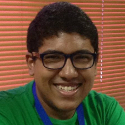
\includegraphics[scale=0.15]{curriculumvitae.jpg}
\end{minipage}
\vspace{1em}

\begin{cvlist}{Experiencia}
\item[{\parbox[t]{6em}{\textit{\large{May 2018\\present}}}}]{
	\parbox[t]{\linewidth}{
		\textbf{\href{http://leadboxhq.com}{Leadbox}} --- Maracay, Venezuela\\
		\textit{Full Stack Developer}\\
		\footnotesize{Mantenimiento y desarrollo de aplicaciones de plataforma para automatización de procesos. Aplicaciones web basadas en Angular.}
	}
}
\item[{\parbox[t]{6em}{\textit{\large{Jul 2017\\May 2018}}}}]{
	\parbox[t]{\linewidth}{
		\textbf{\href{https://guayoyolabs.com}{Guayoyo Labs}} --- Maracay, Venezuela\\
		\textit{Desarrollador Python}\\
		\footnotesize{Mejoras y nuevas funcionalidades para HowlerMonkey, un software para reportar y gestionar vulnerabilidades de seguridad.}
	}
}
\item[{\parbox[t]{6em}{\textit{\large{Feb 2016\\Dic 2016}}}}]{
	\parbox[t]{\linewidth}{
		\textbf{\href{https://www.vauxoo.com}{Vauxoo}} --- Valencia, Venezuela\\
		\textit{Desarrollador Python}\\
		\footnotesize{Desarrollo y mantenimiento de m\'odulos Odoo e im\'agenes Docker.}
	}
}
\item[{\parbox[t]{6em}{\textit{\large{Sep 2014\\May 2015}}}}]{
	\parbox[t]{\linewidth}{
		\textbf{\href{http://www.grupo361.com}{Grupo 361}} --- Maracay, Venezuela\\
		\textit{Ingeniero de Software}\\
		\footnotesize{Desarrollo de frontends y backends para portales de marketing.}
	}
}
\item[{\parbox[t]{6em}{\textit{\large{Nov 2009\\Jul 2014}}}}]{
	\parbox[t]{\linewidth}{
		\textbf{\href{https://www.cnti.gob.ve}{Centro Nacional de Tecnolog\'ias de Informaci\'on}} --- Caracas, Venezuela\\
		\textit{Administrador de Plataforma Tecnol\'ogica}\\
		\footnotesize{Desarrollo del Sistema Operativo Canaima GNU/Linux. Dise\~no e implementaci\'on de soluciones inform\'aticas en Software Libre. Administraci\'on de Servicios. Soporte de alto nivel.}
	}
}
\item[{\parbox[t]{6em}{\textit{\large{Nov 2008\\Nov 2009}}}}]{
	\parbox[t]{\linewidth}{
		\textbf{\href{https://www.netuno.net}{NETUNO}} --- Maracay, Venezuela\\
		\textit{T\'ecnico de Levantamiento}\\
		\footnotesize{Dise\~no de Proyectos para la creaci\'on y ampliaci\'on de Redes Coaxiales para voz, datos y TV bajo el est\'andar DOCSIS. Supervisi\'on de la construcci\'on de Redes H\'ibridas. Levantamiento de informaci\'on en sitio. Diagramaci\'on con Autocad. Gesti\'on de Materiales y Supervisi\'on de Contratistas.}
	}
}
\item[{\parbox[t]{6em}{\textit{\large{Otra\\experiencia}}}}]{
	\parbox[t]{\linewidth}{
		\footnotesize{Freelancer en Upwork (mayormente desarrollo en Python), Profesor en la Universidad Nacional Experimental de la Fuerza Armada.}
	}
}
\end{cvlist}

\begin{cvlist}{Formaci\'on}
\item[{\parbox[t]{6em}{\textit{\large{2011}}}}]{
	\parbox[t]{\linewidth}{
		\textbf{Centro Nacional de Adistramiento} --- Caracas, Venezuela\\
		\textit{Administraci\'on del tiempo y productividad laboral} --- 16 Horas\\
		\footnotesize{T\'ecnicas organizativas, trabajo en equipo, cooperaci\'on y complementariedad, establecimiento de prioridades, cronogramas de actividades, valoraci\'on del tiempo.}
	}
}
\item[{\parbox[t]{6em}{\textit{\large{2011}}}}]{
	\parbox[t]{\linewidth}{
		\textbf{Centro Nacional de Tecnolog\'ias de la Informaci\'on} --- Caracas, Venezuela\\
		\textit{Python avanzado} --- 32 Horas\\
		\footnotesize{Estructuras, entornos virtuales, versionamiento, reStructuredText, Sphinx, Django, Sqlite, GUI (pyGTK, pyQT), iteradores, generadores, decoradores, pruebas unitarias.}
	}
}
\item[{\parbox[t]{6em}{\textit{\large{2011}}}}]{
	\parbox[t]{\linewidth}{
		\textbf{Centro Nacional de Tecnolog\'ias de la Informaci\'on} --- Caracas, Venezuela\\
		\textit{Python b\'asico} --- 16 Horas\\
		\footnotesize{Int\'erprete, librer\'ia est\'andar, funciones b\'asicas, tipos de datos, m\'odulos, ciclos, interacci\'on con el usuario y el sistema operativo, formato de resultados, tratamiento de errores.}
	}
}
\item[{\parbox[t]{6em}{\textit{\large{2011}}}}]{
	\parbox[t]{\linewidth}{
		\textbf{Fundaci\'on Hoatzin} --- Caracas, Venezuela\\
		\textit{Administraci\'on de sitios en Plone con Cyn.in} --- 40 Horas\\
		\footnotesize{Instalaci\'on de Plone con Unified Installer y zc.buildout. Configuraci\'on, apariencia, roles de usuario, instalaci\'on de productos, Zope y ZODB.}
	}
}
\item[{\parbox[t]{6em}{\textit{\large{2009}}}}]{
	\parbox[t]{\linewidth}{
		\textbf{Universidad Nacional Experimental de la Fuerza Armada} --- Maracay, Venezuela\\
		\textit{Ingeniero de Telecomunicaciones}\\
		\footnotesize{Dise\~no, desarrollo, implementaci\'on y depuraci\'on de sistemas de comunicaciones el\'ectricos, electr\'onicos, electromagn\'eticos u \'opticos.}
	}
}
\end{cvlist}

\begin{cvlist}{Conferencias}
\item[{\parbox[t]{6em}{\textit{\large{2018}}}}]{
	\parbox[t]{\linewidth}{
		\textbf{Debian Day} --- INCES, Maracay, Venezuela\\
		\textit{Ponente} --- El Mundo Interno del Programador
	}
}
\item[{\parbox[t]{6em}{\textit{\large{2012}}}}]{
	\parbox[t]{\linewidth}{
		\textbf{FLISOL} --- UNEFA, Maracaibo, Venezuela\\
		\textit{Ponente} --- ¿C\'omo desarrollar para Canaima GNU/Linux?
	}
}
\item[{\parbox[t]{6em}{\textit{\large{2012}}}}]{
	\parbox[t]{\linewidth}{
		\textbf{6ta Cayapa Canaima} --- UNELLEZ, Barinas, Venezuela\\
		\textit{Desarrollador}
	}
}
\item[{\parbox[t]{6em}{\textit{\large{2012}}}}]{
	\parbox[t]{\linewidth}{
		\textbf{DebConf12} --- Managua, Nicaragua\\
		\textit{Ponente} --- Haciendo distribuciones derivadas con Canaima Semilla
	}
}
\item[{\parbox[t]{6em}{\textit{\large{2011}}}}]{
	\parbox[t]{\linewidth}{
		\textbf{7mo Congreso Nacional de Software Libre} --- Barquisimeto, Venezuela\\
		\textit{Ponente} --- Canaima 3.0: ¿Qu\'e hay de nuevo?
	}
}
\item[{\parbox[t]{6em}{\textit{\large{2011}}}}]{
	\parbox[t]{\linewidth}{
		\textbf{FLISOL} --- M\'erida, Venezuela\\
		\textit{Ponente} --- Canaima 3.0: ¿Qu\'e hay de nuevo?
	}
}
\item[{\parbox[t]{6em}{\textit{\large{2011}}}}]{
	\parbox[t]{\linewidth}{
		\textbf{7mo D\'ia Debian} --- Caracas, Venezuela\\
		\textit{Ponente} --- Haciendo distribuciones derivadas con Canaima Semilla
	}
}
\item[{\parbox[t]{6em}{\textit{\large{2011}}}}]{
	\parbox[t]{\linewidth}{
		\textbf{TIL para Vivir Viviendo} --- Caracas, Venezuela\\
		\textit{Ponente} --- ¿Como hacer un sabor de Canaima?
	}
}
\item[{\parbox[t]{6em}{\textit{\large{2011}}}}]{
	\parbox[t]{\linewidth}{
		\textbf{5ta Cayapa Canaima} --- Cuman\'a, Venezuela\\
		\textit{Desarrollador}
	}
}
\item[{\parbox[t]{6em}{\textit{\large{2010}}}}]{
	\parbox[t]{\linewidth}{
		\textbf{3ra Cayapa Canaima} --- UCLA, Barquisimeto, Venezuela\\
		\textit{Ponente/Desarrollador} --- Eficiencia de contenidos con PHP
	}
}
\end{cvlist}

\begin{cvlist}{Habilidades}
\item[\textit{\large{Idiomas}}]{Espa\~nol, Ingl\'es}
\item[\textit{\large{Programaci\'on}}]{C, C++, Python, Shell script, Make, PHP, Javascript, TypeScript, VimL.}
\item[\textit{\large{Web}}]{Jekyll, Django, Flask, jQuery, AnimeJS, Angular, Vue.js, Node.js, Gulp.}
\item[\textit{\large{DevOps}}]{LXC, Vagrant, Docker, Qemu, Virtualbox, Git, Fabric, Ansible, Travis CI, Circle CI.}
\item[\textit{\large{Diagramaci\'on}}]{Markdown, reStructuredText, \LaTeX.}
\item[\textit{\large{Otros}}]{
	Generaci\'on de paquetes instalables, kernels personalizados e im\'agenes instalables para distribuciones GNU/Linux.\\
}
\end{cvlist}

\end{cv}
\end{document}
